\begin{frame}{Akash feedback on 12.09.2018}
\begin{itemize}
\item Check if there is a distinguishing input between the key returned by SAT-attack and the combinational part of the key returned by our method ?
\item \alert{Orthogonal method} : After applying corresponding keys, check if both circuits are \alert{formally equivalent}, to original circuit. 
	\begin{itemize}
		\item ./lcmp ../benchmarks/original/c880.bench ../benchmarks/rnd/c880$\_$enc50.bench key=000000110011111011100110110100001001000100000001000010111010001100111111100100001101000010111000010000010011110000111111011001010000001110110011101011111010010100010101110000010110000110000101

The output will be the string 'equivalent' if the correct key is provided. If not, the utility will output the string 'different'. The above command should produce the output 'equivalent'. If any of the key bits are changed, it is very likely that the utility will output 'different'.
	\end{itemize}
\end{itemize}
\end{frame}

\begin{frame}{Next steps}
	\begin{itemize}
		\item Need \alert{separate} combinational netlists for \alert{scan-mode} (effect of XOR gates along the scan-chain) and \alert{functional-mode} (effect of XOR gates of capture flops). 
		\item In fact, some gates in scan-mode netlist can be removed to arrive at the functional-mode netlist. 
	\end{itemize}
\end{frame}

\begin{frame}{ISCAS85 circuits summary}
\begin{itemize}
\item \texttt{c432} : 27-channel interrupt controller (no XOR chains at primary outputs)
\item \texttt{c880} : 8-bit ALU
%\item \texttt{c2670}: 12-bit ALU and controller
%\item \texttt{c3540}: 8-bit ALU
\item \texttt{c6288}: 16-bit multiplier
\item \texttt{c499/c1355} : 32-bit SEC circuit
\item \texttt{c1908}: 16-bit SEC/DED circuit
\item \texttt{c7552}: 32-bit adder/comparator
\item \texttt{c5315}: 9-bit ALU
\end{itemize}
\end{frame}

\begin{frame}{\texttt{c880} XOR chains}
       \begin{figure}
                \begin{center}
                \label{fig:c880-c-l}
                \caption{\texttt{c880} XOR chains at primary outputs}
                        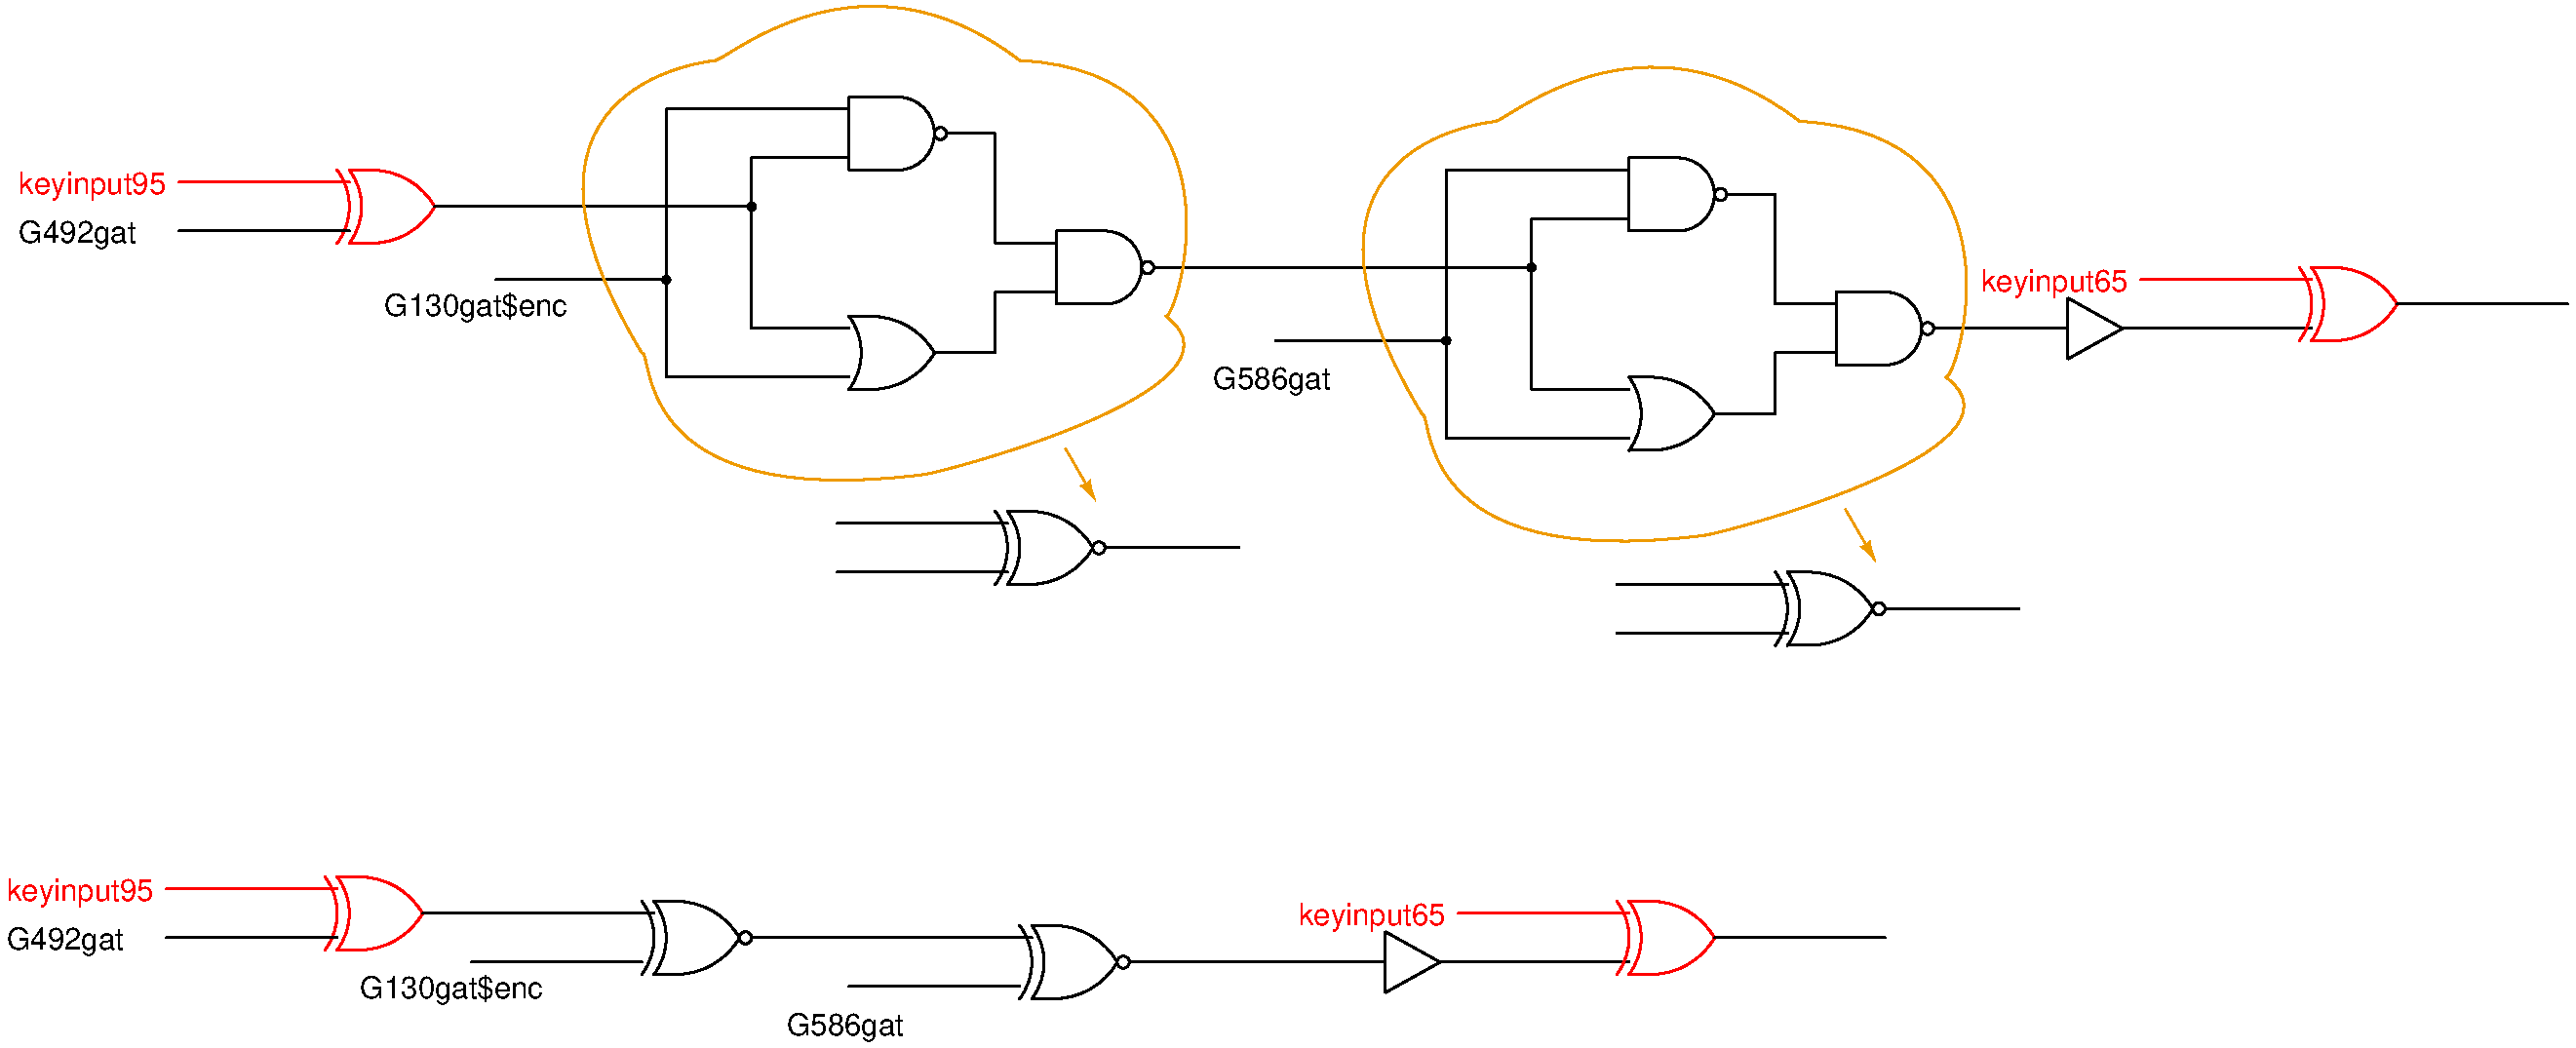
\includegraphics[scale=0.2]{fig/c880-xor-chains.pdf}
                \end{center}
        \end{figure}

\end{frame}

\begin{frame}{\texttt{c6288} XOR chains}
       \begin{figure}
                \begin{center}
                \label{fig:c6288-c-l}
                \caption{\texttt{c6288} XOR chains at primary outputs}
                        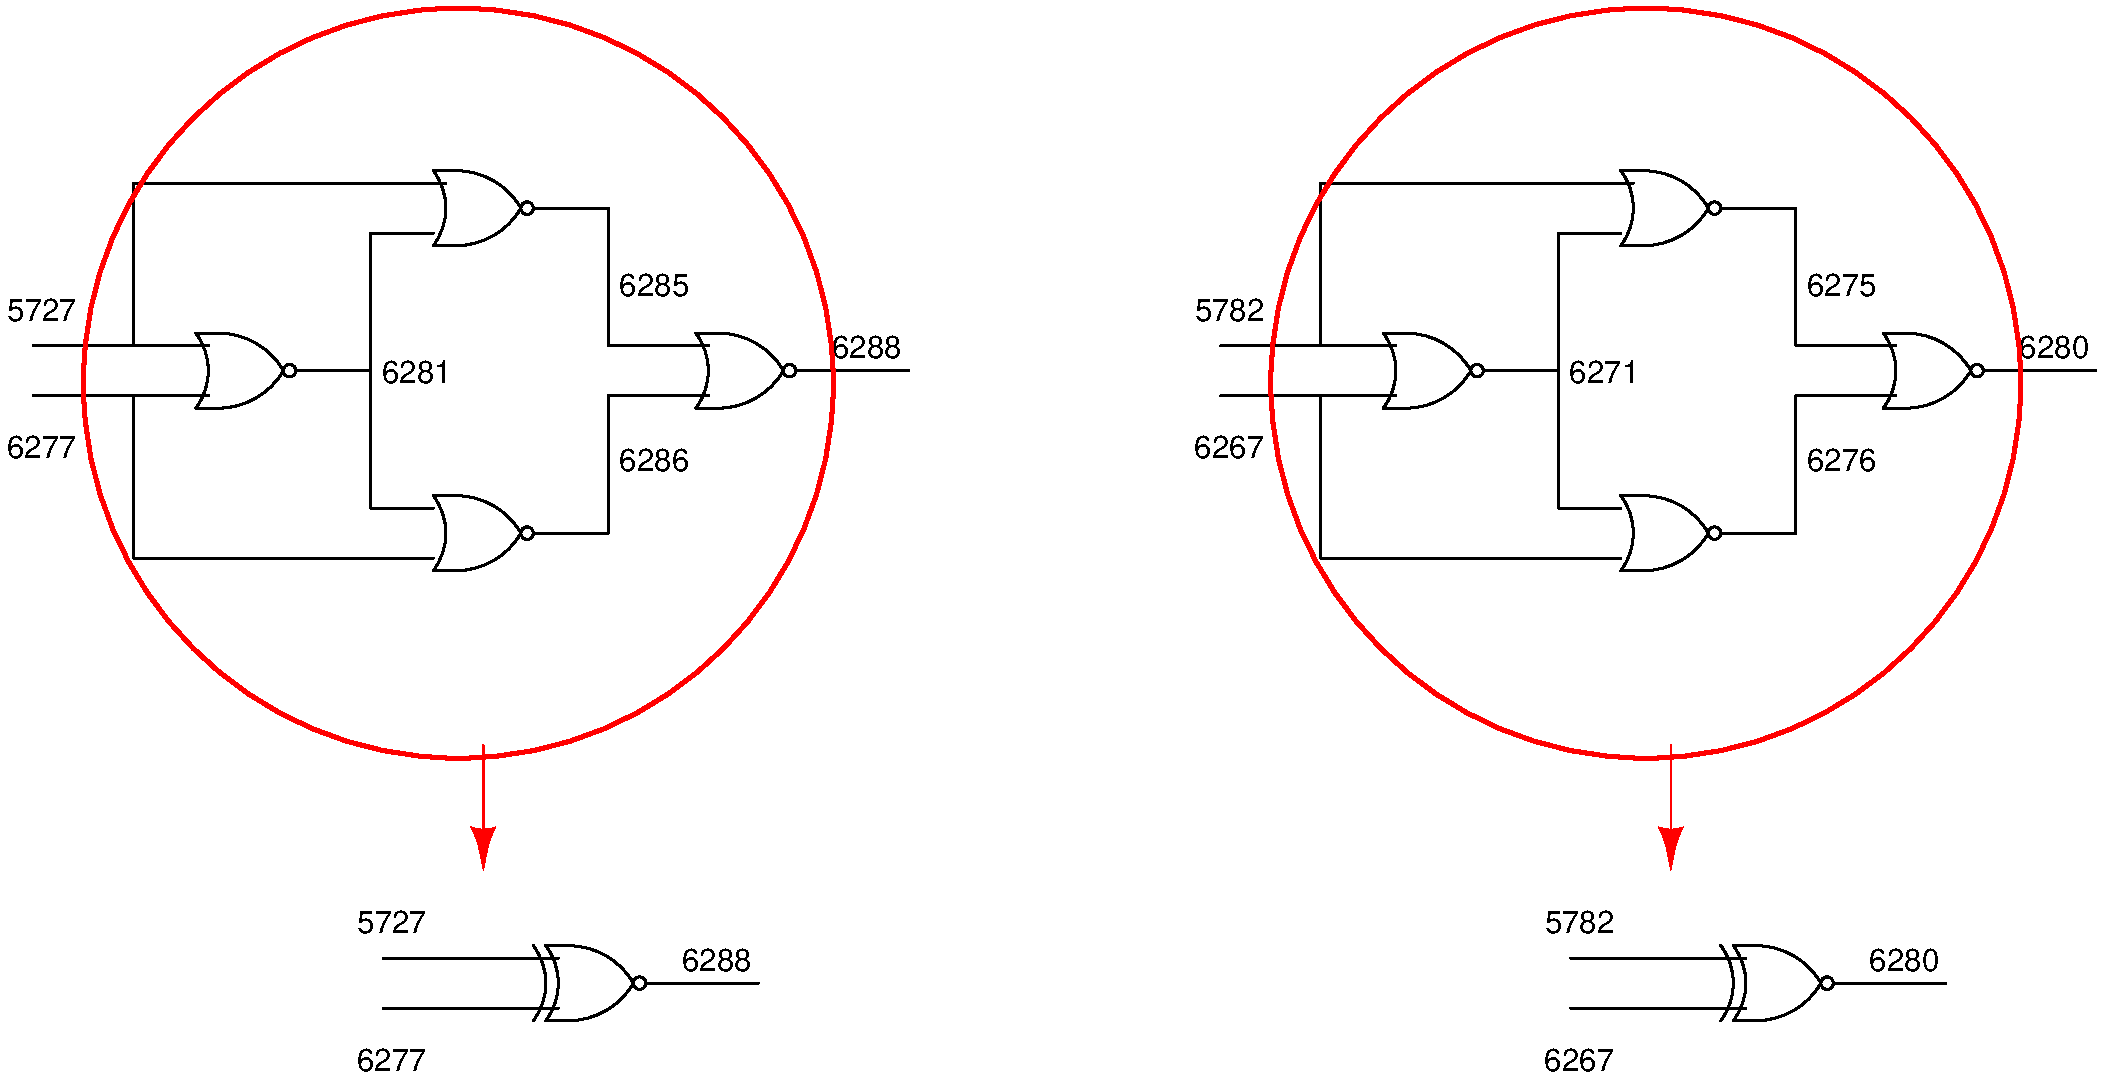
\includegraphics[scale=0.2]{fig/c6288-xor-chains.pdf}
                \end{center}
        \end{figure}

\end{frame}

\begin{frame}{\texttt{c6288} XOR chains}
       \begin{figure}
                \begin{center}
                \label{fig:c6288-c-l}
                \caption{\texttt{c6288} XOR chains at primary outputs}
                        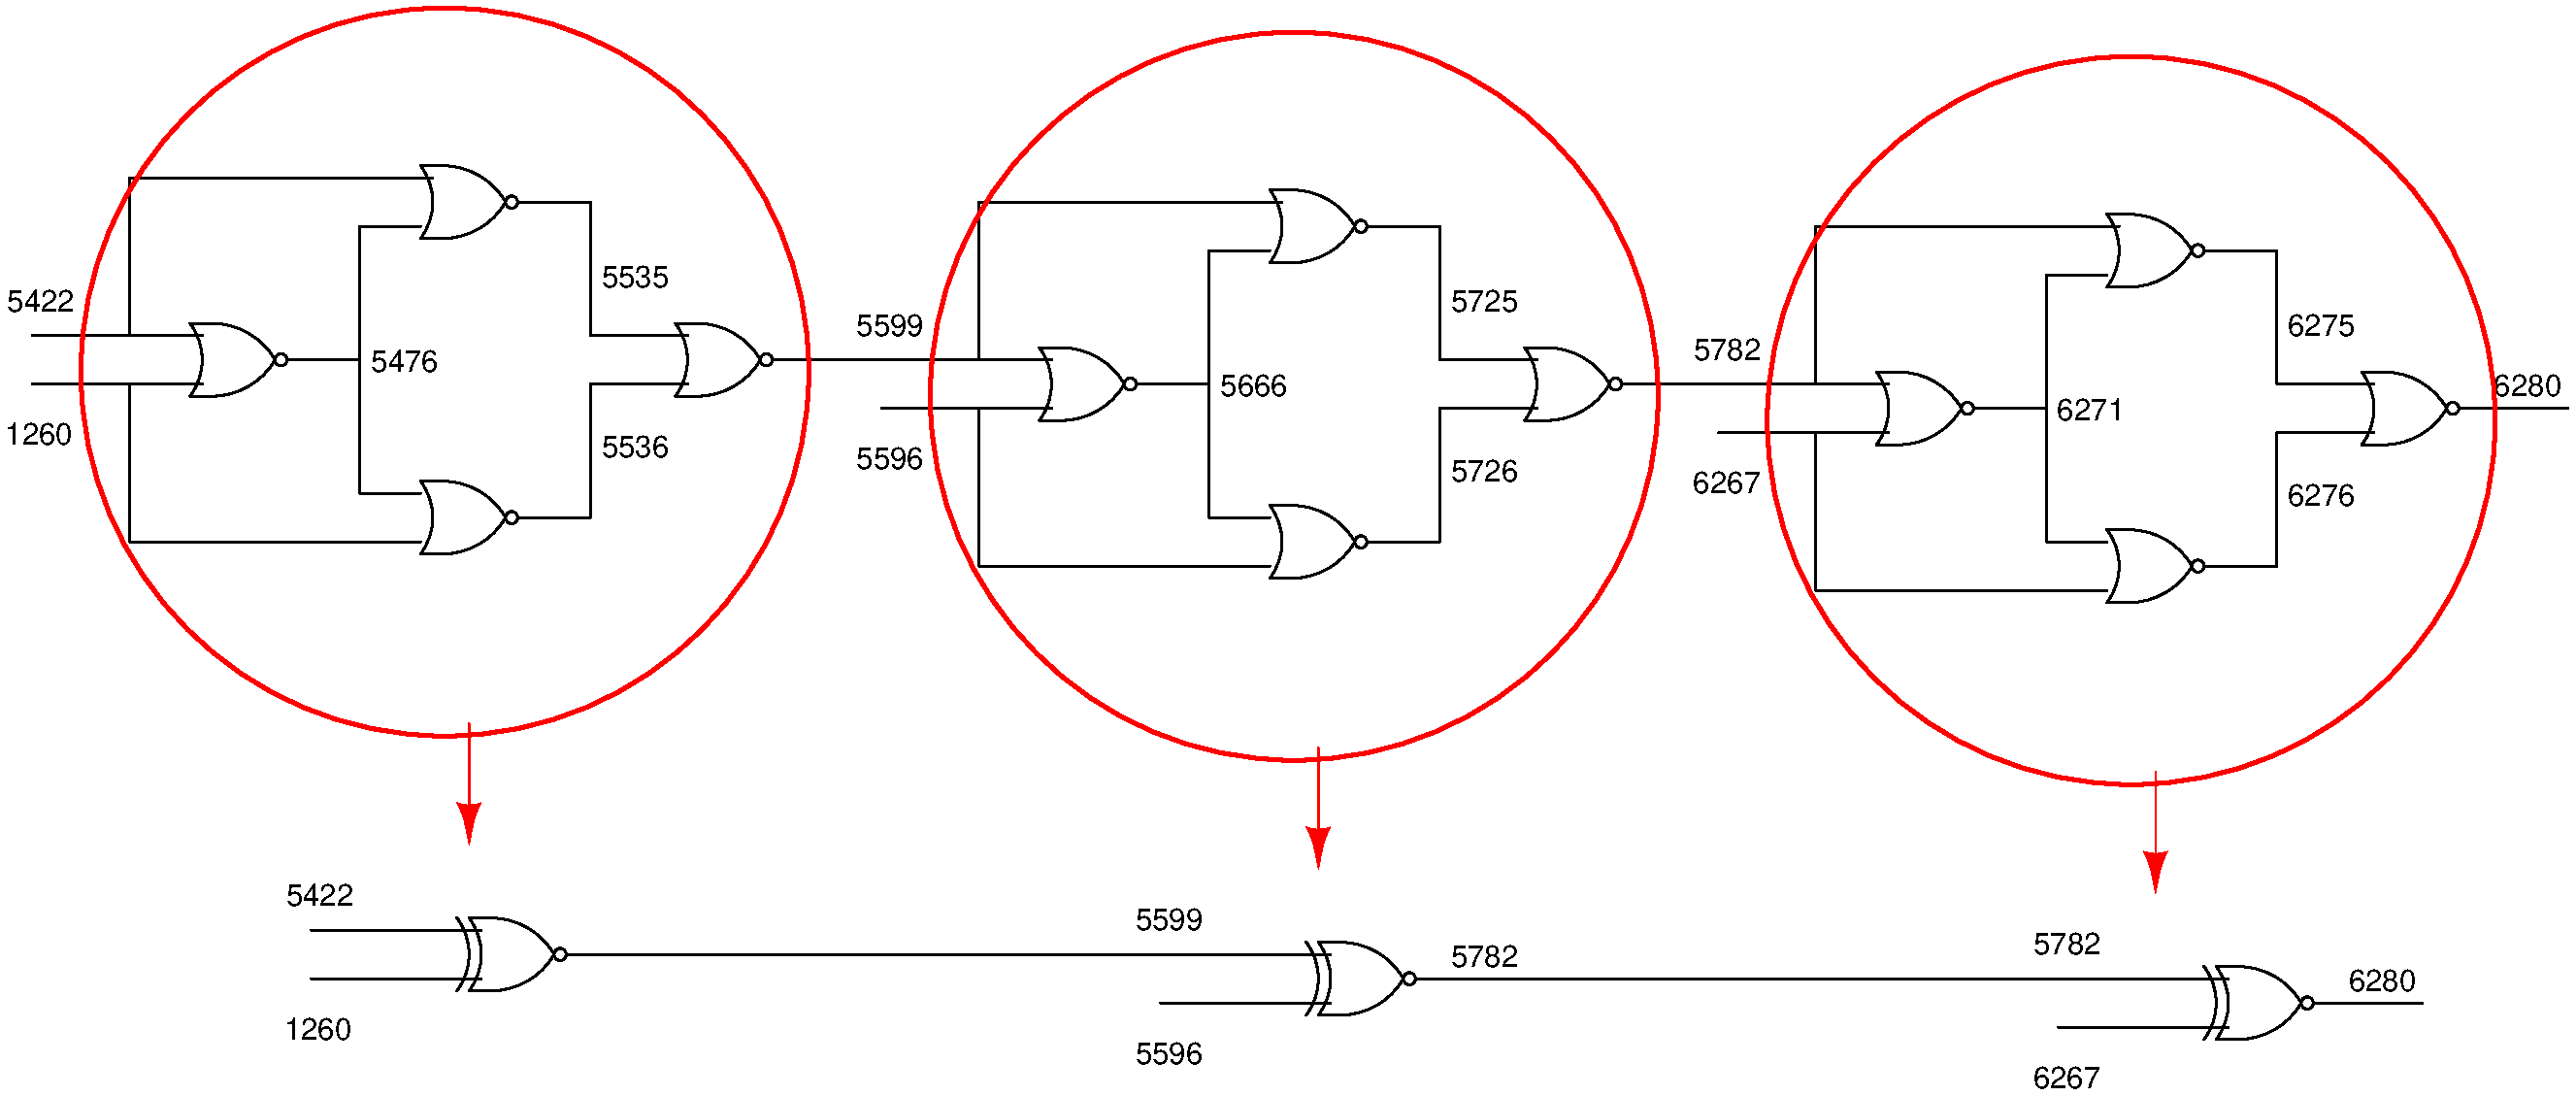
\includegraphics[scale=0.2]{fig/c6288-xor-chains-2.pdf}
                \end{center}
        \end{figure}

\end{frame}

\begin{frame}{\texttt{c499} XOR chains}
       \begin{figure}
                \begin{center}
                \label{fig:c499-c-l}
                \caption{\texttt{c499} XOR chains at primary outputs}
                        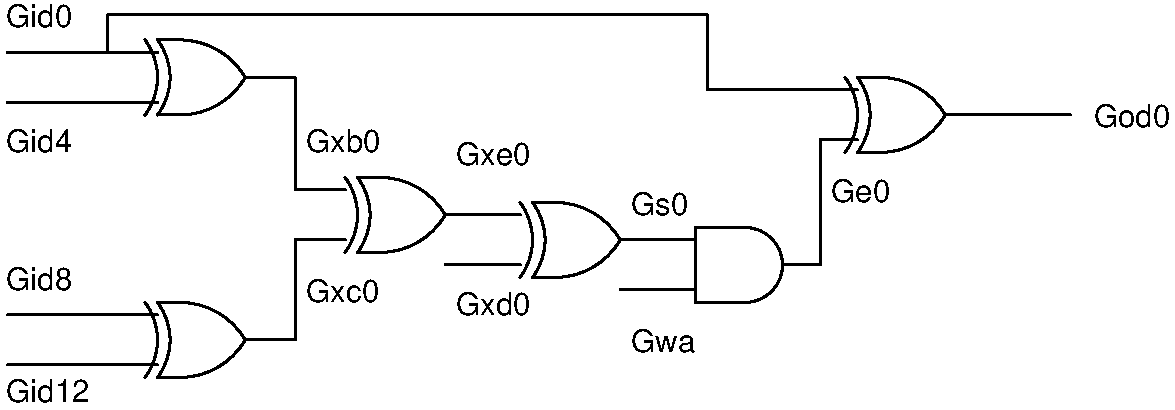
\includegraphics[scale=0.2]{fig/c499-xor-chains.pdf}
                \end{center}
        \end{figure}

\end{frame}



\begin{frame}{\texttt{c499} XOR chains}
       \begin{figure}
                \begin{center}
                \label{fig:c499-c-l}
                \caption{\texttt{c499} XOR chains at primary outputs}
                        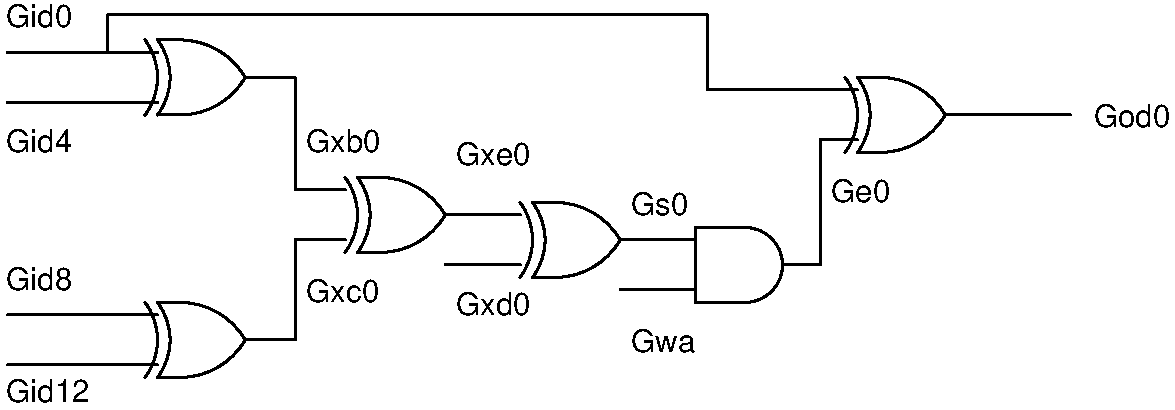
\includegraphics[scale=0.2]{fig/c499-xor-chains.pdf}
                \end{center}
        \end{figure}

\end{frame}

\begin{frame}{\texttt{c1355} XOR chains}
       \begin{figure}
                \begin{center}
                \label{fig:c1355-c-l}
                \caption{\texttt{c1355} XOR chains at primary outputs}
                        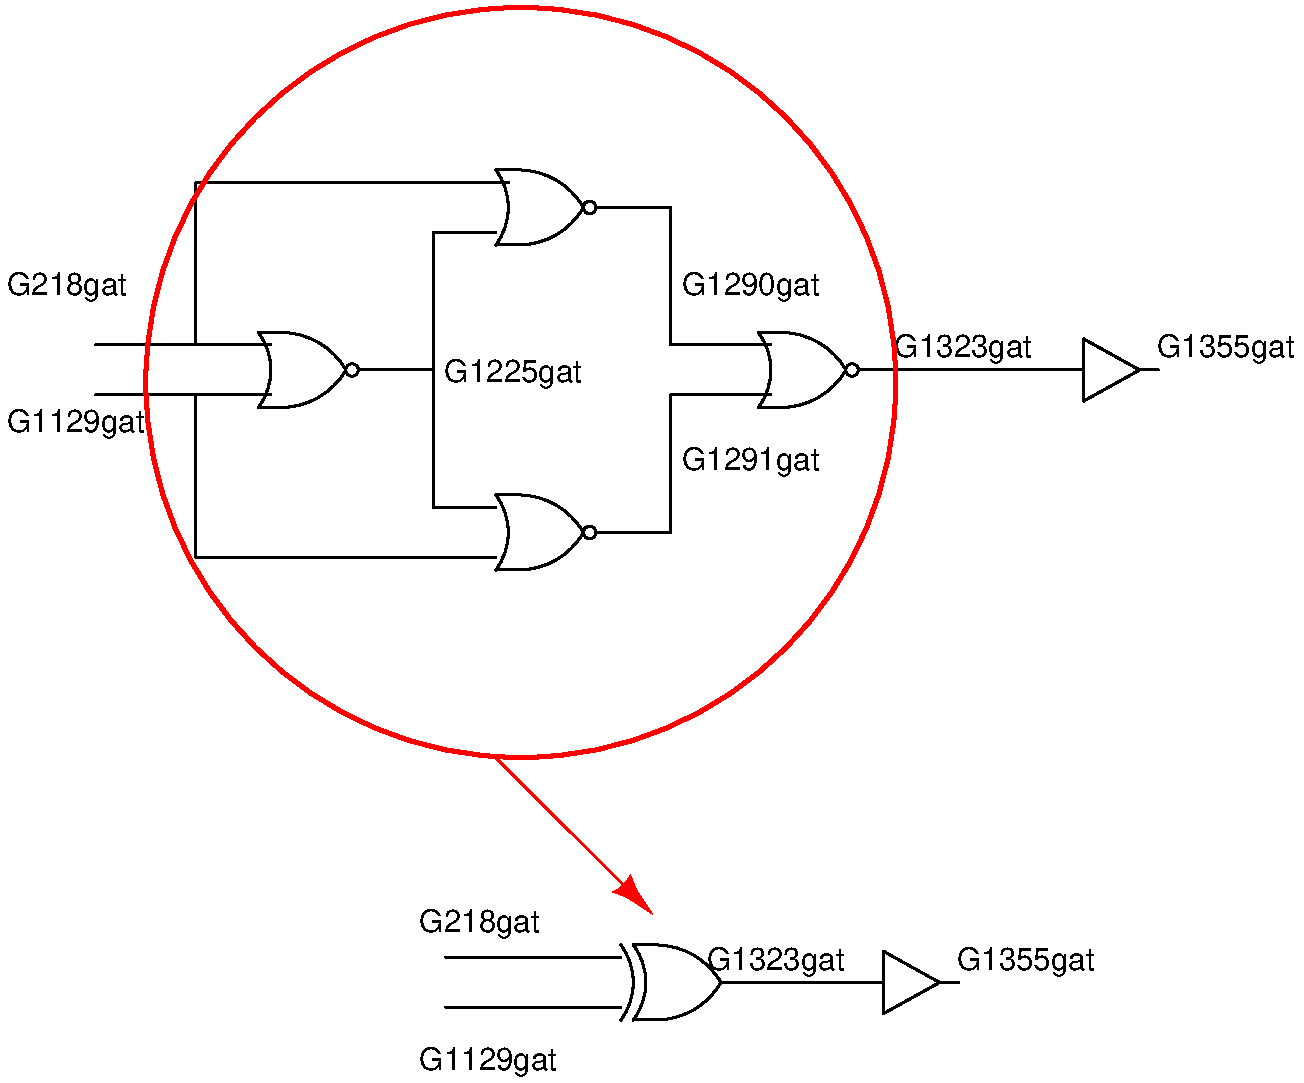
\includegraphics[scale=0.2]{fig/c1355-xor-chains.pdf}
                \end{center}
        \end{figure}

\end{frame}

\begin{frame}{\texttt{c7552} XOR chains}
       \begin{figure}
                \begin{center}
                \label{fig:c7552-c-l}
                \caption{\texttt{c7552} XOR chains at primary outputs}
                        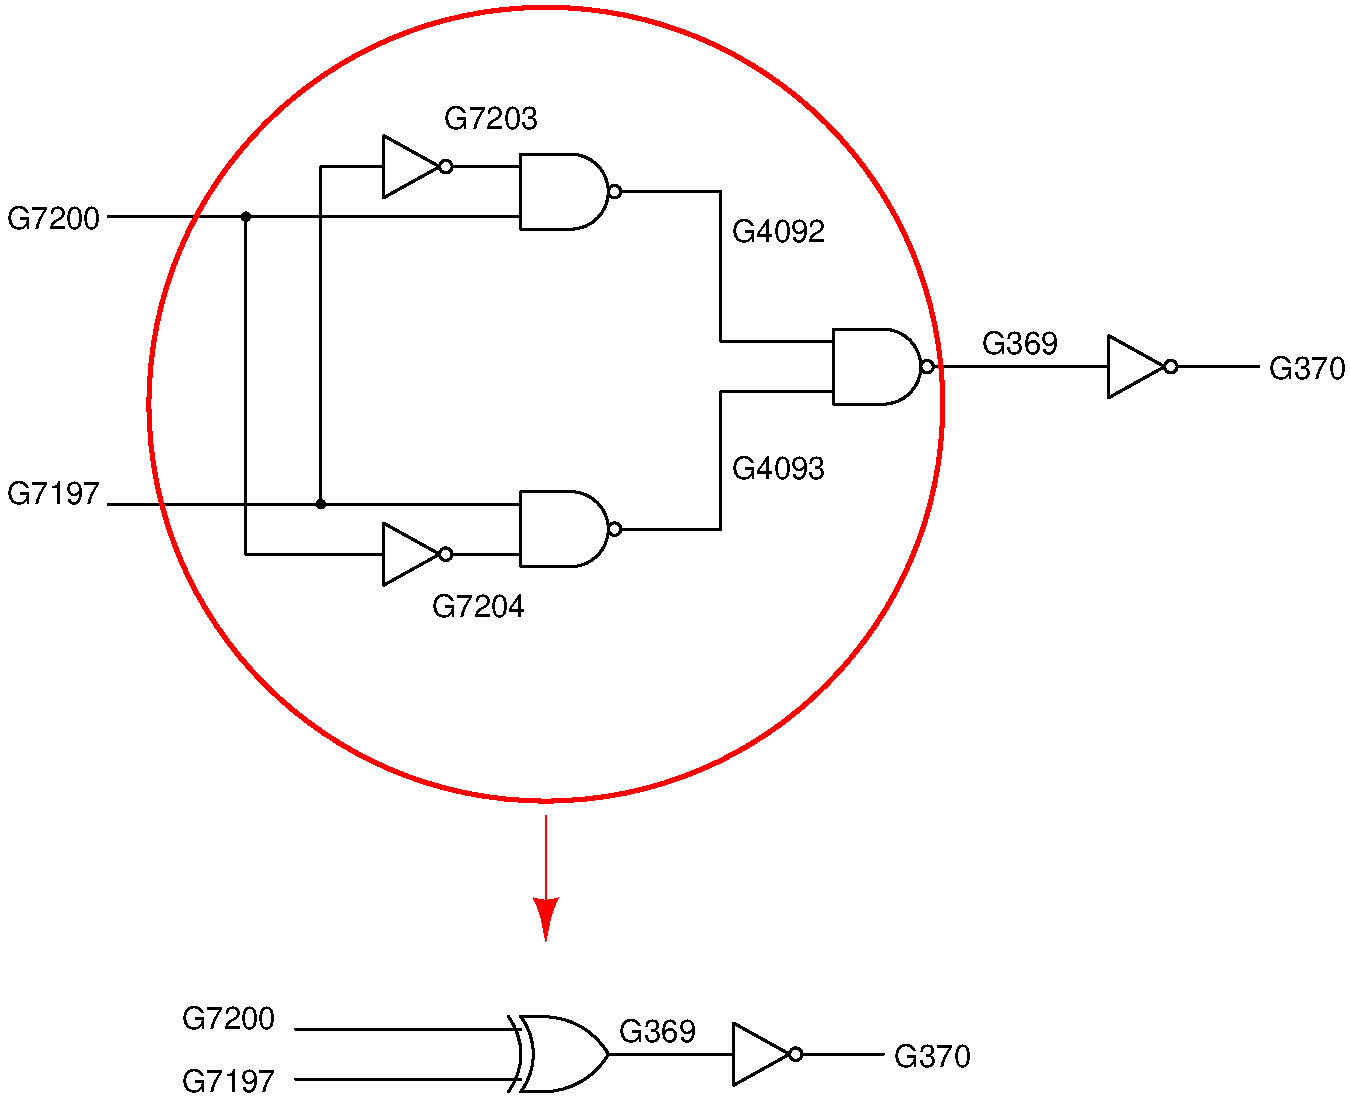
\includegraphics[scale=0.2]{fig/c7552-xor-chains.pdf}
                \end{center}
        \end{figure}

\end{frame}

\begin{frame}{\texttt{c1908} XOR chains}
       \begin{figure}
                \begin{center}
                \label{fig:c1908-c-l}
                \caption{\texttt{c1908} XOR chains at primary outputs}
                        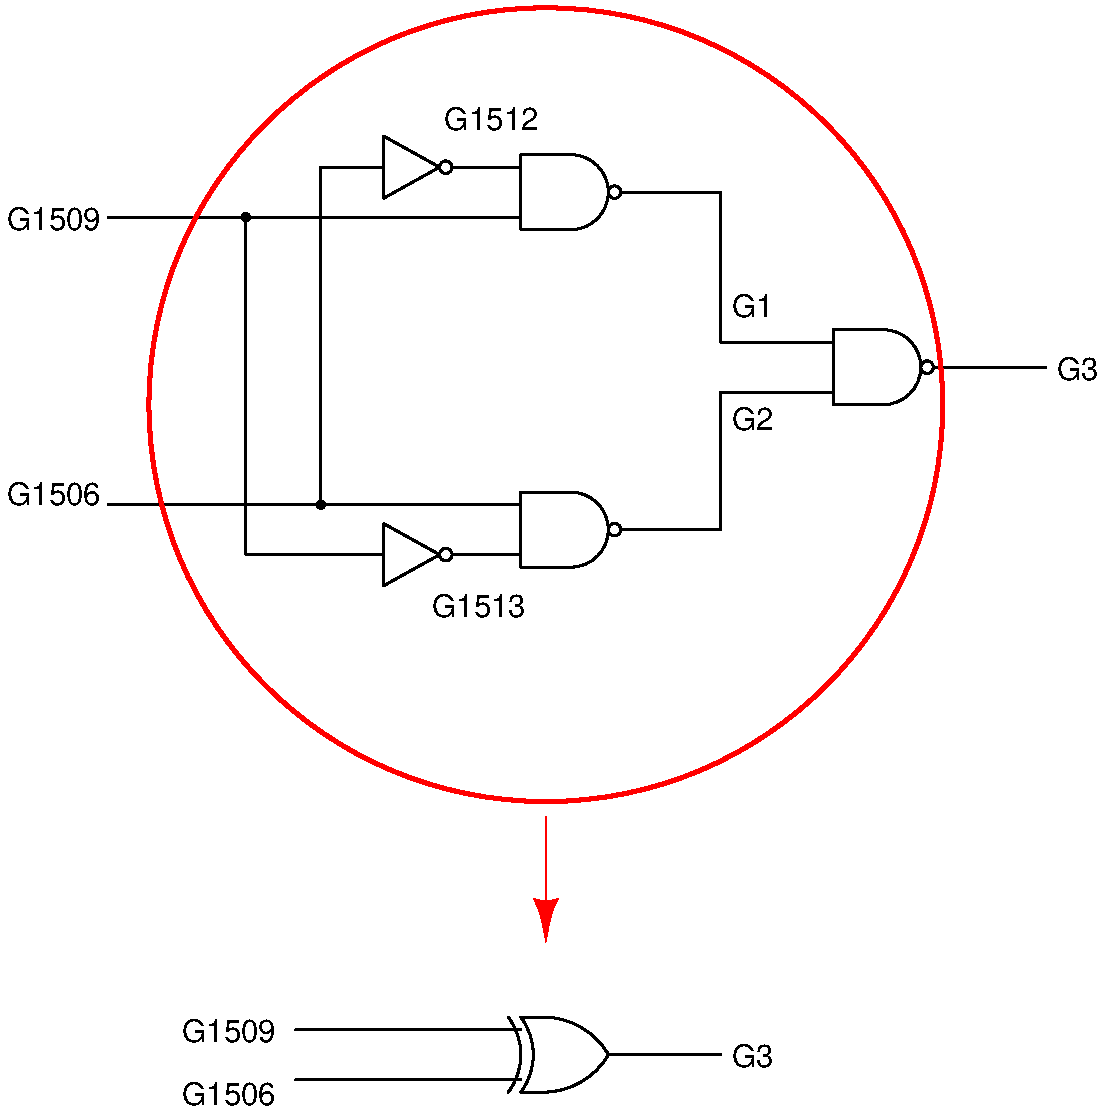
\includegraphics[scale=0.2]{fig/c1908-xor-chains.pdf}
                \end{center}
        \end{figure}

\end{frame}

\begin{frame}{\texttt{c5315} XOR chains}
       \begin{figure}
                \begin{center}
                \label{fig:c5315-c-l}
                \caption{\texttt{c5315} XOR chains at primary outputs}
                        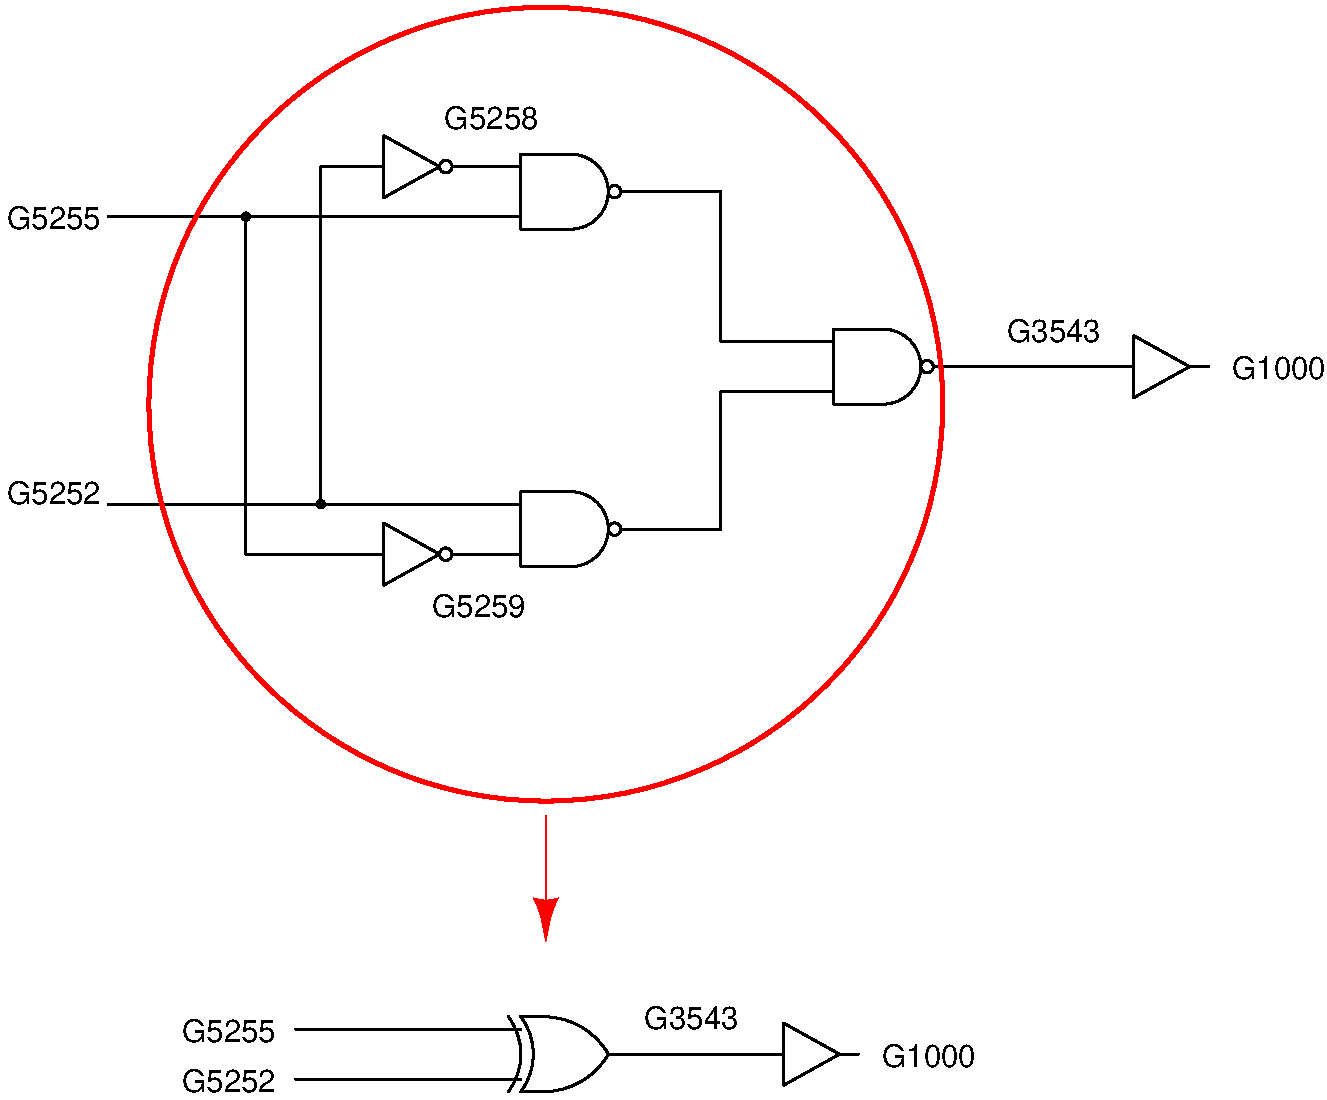
\includegraphics[scale=0.2]{fig/c5315-xor-chains.pdf}
                \end{center}
        \end{figure}

\end{frame}
